\documentclass[11pt, oneside]{article}   	% use "amsart" instead of "article" for AMSLaTeX format
\usepackage{geometry}                		% See geometry.pdf to learn the layout options. There are lots.
\geometry{letterpaper}                   		% ... or a4paper or a5paper or ... 
%\geometry{landscape}                		% Activate for for rotated page geometry
%\usepackage[parfill]{parskip}    		% Activate to begin paragraphs with an empty line rather than an indent
\usepackage{graphicx}				% Use pdf, png, jpg, or eps with pdflatex; use eps in DVI mode
								% TeX will automatically convert eps --> pdf in pdflatex		
\usepackage{xspace}
\usepackage{amssymb}
\usepackage{cite}

\usepackage{xcolor}
\usepackage{xspace}
\def\osprey{{\sc{osprey}}\xspace}
\def\bwmstar{BWM$^*$}
\def\as{\textit{$A^*$}\xspace}
\def\ks{\textit{$K^*$}\xspace}
\def\ka{\textit{$K_a$}\xspace}
\def\bbks{\textit{BBK$^*$}\xspace}


\usepackage{listings}
\lstset{
	basicstyle=\footnotesize
}

\newcommand{\jj}[1]{\if\submissionMode0{\em\color{blue}(JJ: #1)}\else\fi}
\newcommand{\jeff}[1]{\if\submissionMode0{\em\color{blue}(Jeff: #1)}\else\fi}
\newcommand{\suggestion}[1]{\if\submissionMode0{\color{green}\textbf{#1}}\else\fi}


%Submission guidelines for PLoS ONE: http://journals.plos.org/plosone/s/submission-guidelines

\title{{\sc osprey} 3: Open-Source Protein Redesign for You, Refactored, with Powerful New Features}
\author{Mark A. Hallen*, Jeffrey W. Martin*, Adegoke Ojewole$^\dagger$, Jonathan D. Jou$^\dagger$, \\
Anna U. Lowegard, Marcel S. Frenkel, Pablo Gainza, Hunter M. Nisonoff, Aditya Mukund, \\
Siyu Wang, Graham Holt, David Zhou, Elizabeth Dowd, and Bruce R. Donald}
%\date{}							% Activate to display a given date or no date

\begin{document}
\maketitle
*,$^\dagger$ These authors contributed equally
%\section{}
%\subsection{}

\section{Abstract}
We present \osprey 3.0, a new and greatly improved release of the \osprey protein design software.  \osprey 3.0 features a convenient new Python interface, which greatly improves its ease of use.  It is over two orders of magnitude faster than previous versions of \osprey when running the same algorithms on the same hardware.  Moreover, \osprey 3.0 includes several new algorithms, which introduce substantial speedups as well as improved biophysical modeling.  It also includes GPU support, which provides an additional speedup of over an order of magnitude.  Like previous versions of \osprey, \osprey 3.0 offers a unique package of advantages over other design software, including provable design algorithms that account for continuous flexibility during design and model conformational entropy.  Finally, we show here empirically that \osprey 3.0 accurately predicts the effect of mutations on protein-protein binding. \osprey 3.0 is available at https://github.com/donaldlab/OSPREY\_refactor/tree/python as open-source software.    

\section{Introduction}
For over a decade, the {\sc osprey} software package~\cite{OSPREY,minDEE,OSPREY_MIE} has offered the protein design community a unique combination of continuous flexibility modeling, ensemble modeling, and algorithms with provable guarantees.  Having begun as a software release for the $K^*$ algorithm, which approximates binding constants using ensemble modeling, it now boasts a wide array of algorithms found in no other software.  {\sc osprey} has been used in many designs that were empirically successful---\textit{in vitro}~\cite{VRC07_enhance,CFTR,runx1_cbfb,GrsA-LeuA,DHFR-PNAS,GrsA-TyrA,specific_probes} and \textit{in vivo}~\cite{VRC07_enhance,CFTR,runx1_cbfb,DHFR-PNAS} as well as in non-human primates~\cite{VRC07_enhance}.  {\sc osprey}'s predictions have been validated by a wide range of experimental methods, including binding assays, enzyme kinetics and activity assays, in cell assays (MICs, fitness) and viral neutralization, {\em in vivo} studies, and crystal structures~\cite{DHFR-PNAS2, VRC07_enhance}.    

However, as {\sc osprey} grew to include more algorithms and features, the code became increasingly complicated and difficult to maintain.  The growing complexity of the software also hindered its ease-of-use. {\sc osprey} 3.0 represents a complete refactoring of the code, and presents a simpler and more intuitive interface that makes protein redesign much easier than before. The new code organization also facilitates adding new features to the open-source project, both by ourselves and by other contributors.  We have introduced a convenient Python scripting interface and added support for GPU acceleration of the bulk of the computation, allowing designs to be completed much more quickly and easily than in previous versions of {\sc osprey}.  We believe {\sc osprey} 3.0 will be a very useful tool for both developers and users of provably accurate protein design algorithms.  

\jccsubsection{Past successes of {\sc osprey}}

{\sc osprey} has been used for an impressive number of empirically successful designs, ranging from enzyme design to antibody design to prediction of antibiotic resistance mutations.  Notably, {\sc osprey} has been successful in many~\textit{prospective} experimental studies, i.e., studies in which our designed sequences are tested experimentally, thus validating \osprey through use in practice rather than simply through a retrospective comparison of OSPREY calculations to previous experimental results.  {\sc osprey} is most applicable to problems that can be posed in terms of biophysical state transitions like binding, allowing the $K^*$ algorithm and its variants to select the optimal sequence based on an estimate of binding free energy.  But most protein design problems can be posed in this way, sometimes in terms of binding to more than one ligand.  

For example, we have successfully predicted novel resistance mutations to new inhibitors in MRSA (methicillin-resistant~\textit{Staphylococcus aureus}), by searching for sequences that have impaired drug binding compared to wild-type DHFR, but still form the enzyme-substrate complex as usual, allowing catalysis~\cite{DHFR-PNAS,DHFR-PNAS2}.  Our predictions were validated not only biochemically and structurally, but also at an organismal level~\cite{DHFR-PNAS2, mimb_resistance}.  Similarly, we have successfully changed the preferred substrate of an enzyme---the phenylalanine adenylation domain of gramicidin S synthetase---from phenylalanine to leucine by modeling of the two enzyme-substrate complexes, searching for sequences with improved binding to leucine and less to phenylalanine~\cite{GrsA-LeuA}.  The resulting designer enzymes exhibited improved catalysis, and designs changing the specificity from phenlyalanine to several charged amino acids were successful as well.  

Still other successes of {\sc osprey} have involved improving a single binding interaction, like the interaction of the antibody VRC07 with its antigen, the gp120 surface protein of HIV.  Using this approach, we collaborated with the NIH Vaccine Research Center to design a broadly neutralizing antibody (VRC07-523LS) against HIV with unprecedented breadth and potency that is now in clinical trials~\cite{VRC07_enhance,clinical605}.  We also have designed allosteric inhibitors for the leukemia-associated protein-protein interaction between Runx1 and CBF$\beta$~\cite{runx1_cbfb}.  Likewise, we have used {\sc osprey} to develop peptide inhibitors of CAL, a protein involved in cystic fibrosis~\cite{CFTR}.  This is a protein design problem of direct therapeutic significance that consists of optimizing a protein-protein binding interaction.  

In addition, a number of other research groups have successfully used the {\sc osprey} algorithms and software (by themselves) to perform biomedically important protein designs, {\em e.g.,} to design anti-HIV antibodies that are easier to induce \cite{Georgiev:2014aa}; to design a soluble prefusion closed HIV-1-Env trimer with reduced CD4 affinity and improved immunogenicity~\cite{Gwo-yu17}; to design a transmembrane Zn$^{2+}$-transporting four-helix bundle~\cite{Joh14}; to optimize stability and immunogenicity of therapeutic proteins \cite{Parker:2013aa,Salvat:2015aa,Zhao:2015aa}; and to design sequence diversity in a virus panel and predict the epitope specificities of antibody responses to HIV-1 infection~\cite{polyclonal17}.

We believe {\sc osprey} 3.0 will enable an even greater range of successful designs.  


\section{New protein design algorithms in version 3}
\subsection{LUTE: Putting advanced modeling into a form suitable for efficient, discrete design calculations}

{\sc osprey} 3 comes with LUTE~\cite{LUTE_RECOMB}, a new algorithm that addresses two issues with previous versions of {\sc osprey}.  

First, previous versions modeled continuous flexibility by enumerating conformations in order of a~\textit{lower bound} on minimized conformational energy~\cite{minDEE,iMinDEE}.  This approach is often inefficient in that many conformations---possibly even a number exponential in the number of mutable residues---can have lower bounds below the GMEC energy, and thus will all have to be enumerated.  Only a small gain in efficiency is obtained by minimizing the energies of the partial conformations corresponding to nodes of the \as tree~\cite{EPIC}, again because of the gap between lower bounds and actual minimized energies.  LUTE addresses this problem by directly optimizing the minimized energies of full conformations, which are estimated using an expansion in low-order tuples of residue conformations.  Thus, the burden of modeling continuous flexibility is shifted from the combinatorial optimization (\as) step, which has unfavorable asymptotic scaling, to a precomputation step that only scales quadratically with the number of residues.  This precomputation step consists of sampling a ``training set'' of conformations, computing their minimized energies, and then inferring the coefficients of the expansion.  These coefficients can then be used as residue interaction energies in combinatorial search, whether single- or multistate.  The combinatorial search will have the form of a discrete search and thus achieve high efficiency, but will accurately match the results of a continuously flexible search.  

Second, all previous combinatorial protein design algorithms have relied on an explicit decomposition of the energy as a sum of local (e.g., pairwise) terms.  This made design with energy functions that do not have this form difficult. For example, previous use of the Poisson-Boltzmann~\cite{PBSA} energy function, the gold standard of implicit solvent modeling, in design has relied either on~\textit{post-hoc} reranking of a limited number of favorable designs from a calculation based on pairwise energies, which would cause all other designs favored by the Poisson-Boltzmann energetics to be missed, or on a decomposition that is incompatible with continuous flexibility~\cite{PB_pairwise}.  However, LUTE need only calculate the energies of entire conformations in order to infer its coefficients---explicit pairwise energies are not part of this calculation.  Thus LUTE can straightforwardly support general energy functions, and as shown in~\cite{LUTE_RECOMB} it can obtain good fits at least in the case of Poisson-Boltzmann energies.  

{\sc osprey} users can now turn on LUTE for continuously flexible calculations simply by setting the configuration ``useTupExp'' to true.  {\sc osprey} 3 also supports design with Poisson-Boltzmann solvation energy calculations, which use the DelPhi~\cite{OSOR,DelPhi_surface} software for the single-point Poisson-Boltzmann calculations (we ask the user to download DelPhi separately for licensing reasons).  But as an algorithm, LUTE's abilities go well beyond these features---it is a general tool for taking advanced modeling of a single voxel in a system's conformation space and putting into a suitable form for efficient, discrete combinatorial optimization calculations yielding the best design sequence.  As mentioned in~\cite{LUTE_RECOMB}, we are currently working on adding other capabilities like continuous entropy modeling this way.  Moreover, any other researchers who would like to model some phenomenon in protein design, but find it difficult to fit into the usual discrete pairwise framework used in design calculations, are encouraged to try LUTE and {\sc osprey} 3 as a framework for their modeling.  Such improved modeling is essential to increasing the reliability of and range of feasible uses for computational protein design.  
\subsection{CATS: Local backbone flexibility in all biophysically feasible dimensions}

{\sc osprey} pioneered protein design calculations that model local continuous flexibility of sidechains in the vicinity of rotamers in all biophysically feasible dimensions (i.e., the sidechain dihedrals).  This continuous flexibility was often critical in finding optimal sequences~\cite{iMinDEE}, and especially in eliminating artificial steric problems for ideal rotameric conformations that are chosen without consideration of protein context.  In {\sc osprey} 3, we now extend this ability to the backbone: allowing local continuous backbone flexibility in the vicinity of the native backbone in all biophysically feasible dimensions.  

This flexibility is enabled by the CATS algorithm~\cite{CATS}.  CATS uses a new parameterization of backbone conformational space, along with the voxel framework that {\sc osprey} has always included.  It is equivalent to searching over all changes in backbone dihedrals ($\phi$ and $\psi$) subject to keeping the protein conformation constant outside of a specified flexible region. CATS includes an efficient Taylor series-based algorithm for computing atomic coordinates from its new degrees of freedom, enabling efficient energy minimization.  Unlike previous protein design algorithms with backbone flexibility, CATS routinely finds backbone motions on the order of an angstrom while still performing a comprehensive search of its backbone conformation space.  In Ref.~\citen{CATS}, we have shown that backbone flexibility as modeled by CATS is sometimes critical for resolving artificial steric problems and often affects energetics significantly.  

CATS is intended to be run along with {\sc osprey}'s other algorithms, yielding efficient calculations with continuous flexibility in both the sidechains and the backbone. {\sc osprey}'s convenient interface allows a user to add CATS flexibility to a design merely by specifying the start and end points of the backbone segment to be made flexible.  
\def\multisequencebound{MS\xspace}
\def\msbound{\multisequencebound}


\newcommand{\cut}[1]{}

\subsection{\bbks: Efficiently computing the tightest binding sequences from a combinatorially large number of binding partners}
\cut{Although many GMEC-based designs predict sequences which fold and even bind the desired target, proteins do not exist in nature as a single static structure, but instead as thermodynamic ensemble of structures. Protein design algorithms that optimize binding affinity search for sequences whose thermodynamic ensemble energetically favor the desired bound or unbound states over other undesirable states. In doing so, these algorithms search for sequences whose conformational ensemble may contain multiple low-energy conformations in the desired state. Algorithms whose input model accounts for the ensemble-nature of proteins more accurately represent protein flexibility, and can identify sequences with multiple low-energy conformations which GMEC-based algorithms do not model, and would thus overlook.}
In previous versions of \osprey, the \ks algorithm~\cite{K*} modeled an ensemble of Boltzmann-weighted conformations to approximate the Boltzmann-weighted partition function $Z$. It combined dead-end elimination pruning~\cite{DEE} with \as~\cite{DEE,A*} gap-free conformation enumeration to compute provable $\varepsilon$-approximations $Z$ for the protein states of interest. \ks combined these $Z$ scores to approximate the association constant, \ka, as the ratio of $\varepsilon$-approximate partition functions between the bound and unbound states of a protein-ligand complex. Notably, each partition function ratio, called a \ks \emph{score}, is provably accurate with respect to the the biophysical \emph{input model}~\cite{K*,minDEE,iMinDEE}. 
%
\cut{The input model defines the set of allowed amino acid mutations (i.e.~the \emph{sequence space}), structural search space (i.e.~the input structures, and allowed protein flexibility), the optimization objective (e.g.~design for binding affinity), and the energy function~\cite{}.} 
%
Although \ks efficiently and provably approximates while evaluating as little as 3\% of all possible conformations for a given sequence, \ks it must compute a \ks score for each sequence of interest. A long-standing area for potential improvement has therefore been to develop algorithms that efficiently search over \textit{multiple sequences}. All provable ensemble-based algorithms, as well as many heuristic algorithms which optimize binding affinity, are \emph{single-sequence} algorithms, which must compute or bound the binding affinity for each possible sequence. The asymptotic runtime complexity of single-sequence algorithms is therefore linear in the number of possible sequences, and exponential in the number of mutable residues. Therefore, designs with many mutable residues rapidly become intractable when using single-sequence algorithms. To manage the combinatorial explosion of the sequence space, \ks uses its inter-mutation pruning filter to prune sequences whose \ks scores provably cannot be within a user-specified factor of the best sequence encountered thus far. Nevertheless, inter-mutation pruning is applied only \emph{after} \ks initiates binding affinity computation, meaning that \ks must compute the \ks score for each possible sequence.

\osprey 3 provides a new algorithm, \bbks, which overcomes this challenge. \bbks~\cite{BBK*} builds on \ks, and is the first provable, ensemble-based protein design algorithm to run in time sublinear in the number of sequences. The key innovation in \bbks that enables this improvement is the \emph{multi-sequence bound} (\msbound). Rather than compute binding affinity separately for each possible sequence, as single-sequence methods do, \bbks efficiently computes a single provable \ks score upper bound for a combinatorial number of sequences. \bbks uses \msbound bounds to prune a combinatorial number of sequences during the search, entirely avoiding single-sequence computation for all pruned sequences. Indeed, this combinatorial pruning produces a significant empirical runtime speedup: \bbks runs in time sub-linear in the number of sequences. In our experiments, \bbks provably computed the tightest binding sequences while computing \ks scores for up to 10$^5$ fewer sequences than any single-sequence algorithm.

Importantly, \bbks also contains many other powerful algorithmic improvements and implementation optimizations: the parallel architecture of \bbks, which enables concurrent energy minimization, and a novel two-pass partition function bound, which minimizes far fewer conformations while still computing a provable $\varepsilon$-approximation to the partition function. Combined with the combinatorial pruning power of the \msbound bound, \bbks is able to search over sequence spaces two orders of magnitude larger than previously possible with single-sequence \ks, up to 1700 times more efficiently. Not only is \bbks able to provably bound and prune a combinatorial number of suboptimal sequences, \bbks also provably approximates \ks scores for individual sequences up to three orders of magnitude faster than single-sequence \ks. These improvements show that \bbks not only accelerates protein designs that are possible with previous provable algorithms, it also efficiently performs designs that are too large for previous methods.

\jeff{Do we want to mention MPLP here?}
%etc

\section{Performance enhancements in version 3}
\osprey 3.0's code has been heavily optimized to improve single-threaded performance relative to the previous version, \osprey 2.2~\cite{COMETS}. Two main areas have received the most attention and the most improvement in performance so far: \as search speed, and conformation minimization speed.

\osprey uses the \as search algorithm~\cite{DEE/A*} to perform its combinatorial search over sequence and conformational space~\cite{minDEE,iMinDEE,DEEPer}.  The performance of \as search in \osprey depends mostly on the size of the conformation space of the design: the time required for search scales strongly with the number of mutable and flexible residues. Search time is also dependent on the speed at which we can evaluate the energy scoring functions on \as nodes. Optimizations in \osprey 3.0 have dramatically increased the \as node scoring speed, mainly by caching the results of expensive computations and reusing them at different nodes. Many intermediate values used by the \as scoring functions need only be computed once per design. This reduces the cost of node scoring by roughly an order of magnitude. We can also score child nodes differentially against their parent nodes to speed up node scoring. Caching intermediate values during the parent node scoring and using them to simplify child node scoring yields roughly another order of magnitude speedup in \as node scoring. %\jeff{trying to be concise here, hopefully we don't need the mathematical details of these \as scoring functions?}

\osprey 3.0 also includes optimizations to improve the performance of forcefield evaluation and conformation minimization. Conformation minimization is typically the bottleneck in \osprey calculations with continuous flexibility~\cite{minDEE,iMinDEE,DEEPer,CATS}.  The code in \osprey 3.0 that evaluates forcefield energies for a protein conformation has been heavily optimized, although speed gains here over \osprey2 are modest (roughly two-fold), since the original code was already well-optimized in this area. Much larger performance increases were gained by caching forcefield parameters and lists of atom pairs between different conformations to be minimized, which yielded roughly a 10-fold increase in speed. \osprey 3.0 also increases performance by only evaluating forcefield terms involving mutable and/or flexible residues in a design, since interaction energies between other residues will be identical across all sequences and conformations.  Since most designs only model a minority of the residues in a protein as flexible, this can be a substantial improvement. 

Performance comparisons are shown for 45 protein design test cases in Fig.~\ref{fig:2v3} and Table~\ref{table:2v3}.  All these test cases model continuous protein flexibility~\cite{minDEE,iMinDEE,EPIC}, and 18 of them involve provably accurate partition function calculations (see Table~\ref{table:2v3} and Ref.~\citen{EPIC} for details).  To summarize, the optimizations to single-threaded performance described above made \osprey 3.0 on average 461-fold faster than \osprey 2.2 across 29 protein design test cases, and allowed \osprey 3.0 to finish the remaining 16 test cases, which \osprey 2.2 could not finish within a 17-day time limit.  For example, \osprey 2.2 on a Intel Xeon E5-2640 v4 CPU took 49.5 minutes to run a small (6 continuously flexible residues) benchmark sidechain packing problem involving a 114-residue fragment of PDZ3 domain of PSD-95 protein complexed with a 6-residue peptide ligand (PDB ID: 1TP5).  But \osprey 3.0 finished the same design in 7.0 seconds on the same hardware, which is a 424-fold speedup.  

\begin{figure}
\center
\includegraphics[width=4in]{figures/2v3_times.png}
\caption{Runtimes of \osprey 2.2 vs. \osprey 3.0 for 45 protein design test cases (details shown in Table~\ref{table:2v3}), shown on a log scale. Designs that only finished with \osprey 3.0 (given a 17-day time limit) are shown on the right in red.  All test cases involve continuous flexibility~\cite{minDEE,iMinDEE} and minimization-aware DEE~\cite{iMinDEE,EPIC}; 18 involve provably accurate partition function calculations (see Table~\ref{table:2v3} and Ref.~\citen{EPIC} for details).  }
\label{fig:2v3}
\end{figure}

\begin{table}
\caption{
Details of 45 protein design test cases with continuous flexibility run on both \osprey 2.2 and \osprey 3.0.  Test cases primarily adapted from Ref.~\citen{EPIC}.  $^a$ Y indicates a partition function calculation (a subroutine of the $K^*$ algorithm~\cite{K*,minDEE}), which analyzes a thermodynamic ensemble of conformations; N indicates calculation of the single global minimum-energy conformation (GMEC). DNF: Did not finish.  }
\resizebox{\textwidth}{!}{
\begin{tabular}{|p{1.9in}|p{0.5in}|p{0.3in}|p{0.6in}|p{0.75in}|p{0.75in}|p{0.75in}|}
\hline
Protein name	&	PDB code	&	PF?$^a$ 	&	Mutable residue count	&	OSPREY 3.0 time (min)	&	OSPREY 2.2 time (min)	&	Speedup	\\ \hline
Scorpion toxin	&	1AHO	&	N	&	7	&	0.37	&	2.75	&	7.38	\\ \hline
Scorpion toxin	&	1AHO	&	N	&	9	&	0.64	&	6.60	&	10.35	\\ \hline
Scorpion toxin	&	1AHO	&	N	&	12	&	194.71	&	1608.16	&	8.26	\\ \hline
Scorpion toxin	&	1AHO	&	N	&	14	&	287.87	&	2075.04	&	7.21	\\ \hline
Cytochrome c553	&	1C75	&	N	&	6	&	0.28	&	4.30	&	15.19	\\ \hline
Atx1 metallochaperone	&	1CC8	&	N	&	7	&	2.56	&	85.41	&	33.41	\\ \hline
Atx1 metallochaperone	&	1CC8	&	Y	&	7	&	67.12	&	DNF	&	$>$364.72$^\dagger$	\\ \hline
Bucandin	&	1F94	&	N	&	7	&	0.40	&	4.82	&	12.07	\\ \hline
Nonspecific lipid-transfer protein	&	1FK5	&	N	&	6	&	0.03	&	0.78	&	27.34	\\ \hline
Transcription factor IIF	&	1I27	&	N	&	7	&	1.58	&	385.56	&	244.4	\\ \hline
Ferredoxin 	&	1IQZ	&	N	&	9	&	0.16	&	2.45	&	14.92	\\ \hline
Trp repressor 	&	1JHG	&	N	&	7	&	2.88	&	22.50	&	7.8	\\ \hline
Fructose-6-phosphate aldolase 	&	1L6W	&	N	&	6	&	0.23	&	75.97	&	336.22	\\ \hline
Cephalosporin C deacetylase 	&	1L7A	&	N	&	8	&	4.09	&	928.27	&	226.93	\\ \hline
PA-I lectin 	&	1L7L	&	N	&	6	&	0.12	&	6.26	&	52.85	\\ \hline
Phosphoserine phosphatase 	&	1L7M 	&	N	&	7	&	1.13	&	249.33	&	220.11	\\ \hline
alpha-D-glucuronidase 	&	1L8N	&	N	&	5	&	0.13	&	480.13	&	3701.36	\\ \hline
\end{tabular}
}

$^\dagger$ \osprey 2.2 did not finish within the time limit, so we report a lower bound on the speedup: the ratio of the time limit (17 days) to the \osprey 3.0 runtime.   
(Table continues on next page)
\label{table:2v3}
\end{table}

\begin{table}
\resizebox{\textwidth}{!}{
\begin{tabular}{|p{1.9in}|p{0.5in}|p{0.3in}|p{0.6in}|p{0.75in}|p{0.75in}|p{0.75in}|}
\hline
Protein name	&	PDB code	&	PF?$^a$ 	&	Mutable residue count	&	OSPREY 3.0 time (min)	&	OSPREY 2.2 time (min)	&	Speedup	\\ \hline
Dachshund	&	1L8R	&	N	&	8	&	0.19	&	1.41	&	7.62	\\ \hline
Granulysin 	&	1L9L	&	N	&	7	&	0.06	&	1.24	&	20.8	\\ \hline
gamma-glutamyl hydrolase 	&	1L9X	&	N	&	5	&	0.03	&	92.13	&	3507.46	\\ \hline
Ferritin 	&	1LB3 	&	N	&	5	&	0.42	&	23.42	&	55.2	\\ \hline
Cytochrome c 	&	1M1Q 	&	N	&	8	&	1.68	&	357.59	&	213.09	\\ \hline
Hypothetical protein YciI 	&	1MWQ	&	N	&	8	&	0.13	&	3.69	&	28.13	\\ \hline
ygfY	&	1X6I	&	Y	&	14	&	604.71	&	DNF	&	$>$40.48$^\dagger$	\\ \hline
ADAR1 ZB domain	&	1XMK	&	Y	&	15	&	2172.23	&	DNF	&	$>$11.27$^\dagger$	\\ \hline
Histidine triad protein 	&	2CS7	&	Y	&	14	&	2816.56	&	DNF	&	$>$8.69$^\dagger$	\\ \hline
Transcriptional regulator AhrC 	&	2P5K	&	Y	&	11	&	1.18	&	DNF	&	$>$20811.61$^\dagger$	\\ \hline
Scytovirin 	&	2QSK	&	N	&	10	&	10.47	&	164.49	&	15.71	\\ \hline
Scytovirin 	&	2QSK	&	Y	&	10	&	2.54	&	9267.19	&	3651.9	\\ \hline
Hemolysin 	&	2R2Z	&	Y	&	12	&	42.02	&	DNF	&	$>$582.58$^\dagger$	\\ \hline
Putative monooxygenase 	&	2RIL	&	N	&	8	&	18.16	&	15.89	&	0.87	\\ \hline
Putative monooxygenase 	&	2RIL	&	Y	&	8	&	0.23	&	104.77	&	463.18	\\ \hline
alpha-crystallin 	&	2WJ5	&	Y	&	15	&	226.32	&	DNF	&	$>$108.17$^\dagger$	\\ \hline
Cytochrome c555 	&	2ZXY	&	Y	&	14	&	381.39	&	DNF	&	$>$64.19$^\dagger$	\\ \hline
High-potential iron-sulfur protein 	&	3A38	&	Y	&	13	&	65.15	&	DNF	&	$>$375.72$^\dagger$	\\ \hline
ClpS protease adaptor 	&	3DNJ	&	Y	&	12	&	65.04	&	DNF	&	$>$376.4$^\dagger$	\\ \hline
Putative monooxygenase 	&	3FGV	&	Y	&	10	&	1.94	&	DNF	&	$>$12591.94$^\dagger$	\\ \hline
Protein G 	&	3FIL	&	Y	&	14	&	303.81	&	DNF	&	$>$80.58$^\dagger$	\\ \hline
Viral capsid 	&	3G21	&	Y	&	15	&	188.53	&	DNF	&	$>$129.85$^\dagger$	\\ \hline
dpy-30-like protein 	&	3G36	&	N	&	4	&	1.55	&	9.97	&	6.43	\\ \hline
dpy-30-like protein 	&	3G36	&	Y	&	4	&	0.05	&	2.44	&	47.07	\\ \hline
Hfq protein 	&	3HFO	&	Y	&	10	&	6.81	&	DNF	&	$>$3594.09$^\dagger$	\\ \hline
Cold shock protein 	&	3I2Z	&	Y	&	14	&	20.84	&	DNF	&	$>$1174.8$^\dagger$	\\ \hline
HPI integrase	&	3JTZ	&	Y	&	14	&	859.69	&	DNF	&	$>$28.48$^\dagger$	\\ \hline
PSD-95 PDZ3 domain	&	1TP5	&	N	&	6	&	0.12	&	49.50	&	424.29	\\ \hline
\end{tabular}
}
\end{table}


\subsection{GPU acceleration reduces design runtimes}

The vast majority of \osprey runtime in designs with continuous flexibility is spent minimizing protein conformations and conformation fragments. Although the runtimes of sufficiently large designs can be dominated by the exponential-time worst case performance of the A* search phase, if the A* phase can be completed within an acceptable time limit, the merely polynomial-time conformation minimization phase still often dominates the total run time because conformation minimization is a computationally-expensive and time-consuming function {\it per-operation} compared to scoring nodes in the A* tree. In other words, even though we need to do an exponential amount of work to select leaf nodes in the A* tree corresponding to the low-energy conformations of the design, examining A* nodes is relatively inexpensive. Minimizing the conformations associated those same A* leaf nodes to calculate their true forcefield energies is much more expensive, and can take far more time overall. Therefore, methods that increase protein conformation minimization speeds can have a dramatic impact on \osprey runtimes in cases where the A* search time is acceptable.

Much work has been done in the past to optimize \osprey for execution on CPUs, particularly highly multi-core CPUs and even networked clusters of CPU-powered servers \jeff{add some citations here?}. However, modern GPU hardware enables high-performance computation at a fraction of the cost of large CPU clusters, mainly due to the huge video game industry that propels innovation in hardware design and drives down costs. \osprey3 includes GPU programs (called {\it kernels}) built using the CUDA framework that implements the forcefield calculations and local minimization algorithms used in protein redesign. We present performance results of these GPU kernels on various hardware platforms in Figure~\ref{fig:gpu}. Overall, on desktop-class machines, GPU hardware improves minimizations speeds over multi-core CPUs by roughly 12-fold for sufficiently large molecules. On server-class machines, a single GPU is merely about 2.6-fold faster than dual CPUs. These large machines can house more GPUs than CPUs though, so a fully-provisioned server with 4 or even 8 GPUs would likely greatly outperform 2 or even 4 CPUs. \jeff{It's super hard to get good multi-GPU benchmark data on the shared CS machines. Hopefully a speculative statement about multi-GPU performance is good enough here?}

Modern GPU architectures offer thousands of parallel hardware units for calculations, compared to the tens of parallel hardware units in modern CPU architectures. The performance results of the current incarnation of \osprey's GPU kernels indicate that current minimization speeds on GPUs have only begun to scratch the surface of what is possible, particularly for molecules with a small number of atom pairs. It is incredibly likely that future versions of these GPU kernels will offer significantly higher performance on the same hardware -- perhaps allowing minimization speeds many times faster than today's GPU kernels.

\begin{figure}\label{fig:gpu}
\center
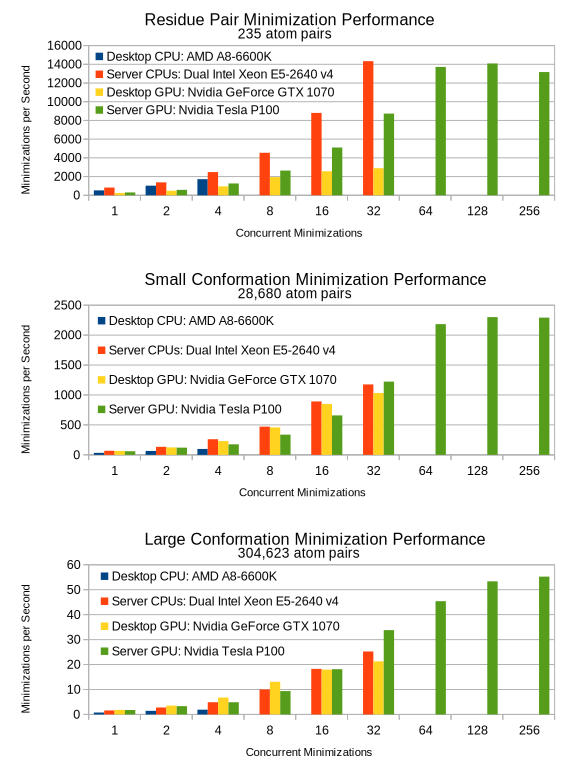
\includegraphics[width=4in]{figures/gpu.pdf}

\jeff{This figure turned out kind of big. Is there room for it? Should we cut some results? Or present them differently?}
\caption{Benchmarks for protein conformation minimization in \osprey3 for various hardware platforms and for molecules of varying size. From smallest to largest: {\bf (top)} a single residue pair used in energy matrix computations, {\bf (middle)} a full protein conformation with a single flexible residue, {\bf (bottom)} a full protein conformation with 20 flexible residues. For CPU hardware, concurrent minimizations correspond to CPU threads. For GPU hardware, concurrent minimizations correspond to {\it streams} defined by the CUDA framework. Faster minimization speeds correspond with faster \osprey runtimes.}
\end{figure}


\section{Python scripting improves ease-of-use}

One of the most visible additions to \osprey 3.0 is the Python application programming interface (API), which allows fine-grained control over design parameters in a streamlined and easy-to-use experience. \osprey 3.0 still supports a command-line interface with configuration files for backwards compatibility, but new development will be focused mostly on the new Python interface. %\jeff{Is this even true? Not entirely sure...} 

The \osprey 3.0 distribution contains a Python module which is installed using the popular package manager {\sc pip}. Once installed, using \osprey 3.0 is as easy as writing a Python script. High-performance computations are still performed in the Java virtual machine to give the fastest runtimes, so Java is still required to run \osprey 3.0, but communication between the Python environment and the Java environment is handled behind-the-scenes, and \osprey 3.0 still looks and feels like a regular Python application.

See Figure~\ref{fig:pythonGMEC} for a complete example of a Python script that performs a very simple design using \osprey 3.0, and Figure~\ref{fig:pythonBBKS} for a slightly more involved design using \bbks~\cite{BBK*} (a new algorithm in \osprey 3.0, described in its own section below).  Figure~\ref{fig:pythonBBKSpic} graphically displays the design setup for the \bbks design.  

\begin{figure}
\vspace{-0.7in}
{\fontfamily{pcr}
	\lstinputlisting[language=Python]{figures/findGMEC.py}
}
\caption{\textbf{A Python script that performs a very simple design in \osprey 3.0.}  The design searches over sequences in which residues A2 and/or A3 of the Atx1 metallochaperone protein (PDB ID: 1CC8)~\cite{1CC8} are mutated; residues A2-A4 (i.e., residue 2-4 of chain A) are all modeled with sidechain flexibility, consisting of a discrete search over the Penultimate rotamer library\cite{penultimate}'s rotamers for the specified amino acid types.  The mutability, flexibility, and starting crystal structure are all specified in the ``define a strand'' section of the code.  Advanced users can also modify the other sections to specify changes from the default search algorithms, energy function, and other modeling assumptions.  This script uses the MPLP algorithm~\cite{MPLP} to reduce the size of the \as search tree~\cite{DEE/A*} used for sequence and conformational search without compromising accuracy; see Ref.~\cite{dynamic_A*} for details.  }
\label{fig:pythonGMEC}
\end{figure}

\begin{figure}
\vspace{-0.7in}
\resizebox{\textwidth}{!}
{\fontfamily{pcr}
	\lstinputlisting[language=Python]{figures/bbkstar.py}
}
\caption{\textbf{A Python script that performs a simple \bbks design in \osprey 3.0.}  This design produces a peptide to bind human fibronectin (the ``ligand strand,'' i.e. chain A) by optimizing a fragment of the protein FnBPA from~\textit{Staphylococcus aureus} (the ``protein strand,'' chain G), which has been crystallized in complex with fibronectin domains (PDB ID: 2RL0~\cite{2RL0}).  As in Fig.~\ref{fig:pythonGMEC}, the script defines the starting crystal structure, mutable residues, and level of mutability and flexibility (here including continuous flexibility) in the form of Python strand objects.   Fig.~\ref{fig:pythonBBKSpic} represents this design graphically.  This design is accelerated by parallelism, running on 4 CPU cores.    }
\label{fig:pythonBBKS}
\end{figure}

\begin{figure}
\includegraphics[width=3.25in]{figures/python_bbks_full.png}\includegraphics[width=3.25in]{figures/python_bbks_zoom.png}
\caption{\textbf{Setup for the Python-scripted \bbks~\cite{BBK*} design described in Fig.~\ref{fig:pythonBBKS}.}  This design starts with the crystal structure (PDB ID: 2RL0~\cite{2RL0}) of a complex between fragments of the protein FnBPA from~\textit{Staphylococcus aureus} (blue ribbons) and human fibronectin (green ribbons), and optimizes binding with respect to the amino acid type of FnBPA residue 649 (magenta), while modeling continuous flexibility in several surrounding sidechains (orange).  The full complex is shown on the left, while the region surrounding the mutation is shown in detail on the right.  }
\label{fig:pythonBBKSpic}
\end{figure}

\section{Conclusions}
\osprey has long offered unique capabilities to protein designers.  In particular, it has always offered a unique combination of free energy-based modeling, provably accuracy conformational search, continuous flexibility, and efficient search over large sequence spaces.  In \osprey 3.0 we introduced software improvements that will make these algorithms much more practical for the wider design community: performance that is orders of magnitude faster, and a Python interface that makes \osprey much easier to use.  On top of this, we expanded the range of biophysical modeling assumptions that \osprey can accommodate, both in terms of molecular flexibility and energy functions.  We hope this new version will be of significant utility to designers, whether they have used \osprey before or are trying it for the first time.  



\bibliographystyle{plain}
\bibliography{references}


\end{document}  